% Copyright 2013 Nicolai Hähnle <nhaehnle@gmail.com>
%
% This work is licensed under the Creative Commons Attribution-ShareAlike 3.0
% Unported License, see http://creativecommons.org/licenses/by-sa/3.0/
% 
% Among other things, this means that yes, you may take e.g. illustrations from
% the book and use them in your own work. However, (a) you must give proper
% attribution by naming me as its original author and (b) you must make your
% derivative work available under the same or similar license terms.
%
% See the Creative Commons website for the exact licensing terms.

\chapter{Lattice Basics and Minkowski's theorem}

Let us begin with an old question:
\begin{problem}
  When can a natural number $n$ be expressed as the sum of two squares, that is,
  when can we write $n = x^2 + y^2$ where $x$ and $y$ are integers?
\end{problem}
Suppose that $n = ab$, where both $a$ and $b$ are sums of two squares of integers, that is
\begin{align*}
  a &= x^2 + y^2 \\
  b &= z^2 + w^2
\end{align*}
Then
\begin{align*}
  n &= ab \\
    &= (x^2 + y^2)(z^2 + w^2) \\
    &= x^2 z^2 + x^2 w^2 + y^2 z^2 + y^2 w^2 \\
    &= (xz + yw)^2 + (xw - yz)^2
\end{align*}
That is, every product of sums of two squares can be written as a sum of two squares.
This suggests we should focus on indivisible factors, i.e. prime numbers.

\begin{problem}
  \label{problem:prime-sum-of-squares}
  When can a prime $p$ be expressed as the sum of two squares, that is,
  when can we write $p = x^2 + y^2$ where $x$ and $y$ are integers?
\end{problem}
The sum of squares reminds us of Pythagoras' theorem:
\begin{center}
  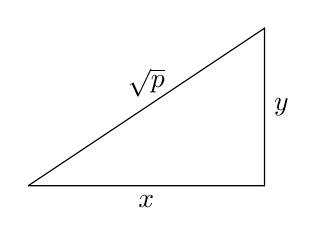
\begin{tikzpicture}
    \draw (0,0) -- node[below] {$x$} (3,0) -- node[right] {$y$} (3,2)-- node[above] {$\sqrt{p}$} (0,0);
  \end{tikzpicture}
\end{center}
We can rephrase Problem~\ref{problem:prime-sum-of-squares}:
For which primes $p$ is there an integer point on the circle of radius $\sqrt{p}$ around the origin?

Geometry alone cannot answer this question. Let us look at some examples:
\[ \mathbf{2}, 3, \mathbf{5}, 7, 11, \mathbf{13}, \mathbf{17}, 19, 23, \mathbf{29}, 31, \mathbf{37}, \mathbf{41}, 43, 47, \mathbf{53}, 59, \mathbf{61}, \dots \]
Ignoring the special case of the rather odd prime $2$,
the primes that can be written as a sum of two squares appear to be exactly those that are congruent to $1$ modulo $4$.
Indeed, $x^2 \equiv 0$ or $1 \pmod{4}$ for all integers $x$, so $x^2 + y^2 \equiv 0, 1, 2 \pmod{4}$.
\begin{fact}
  If $p \equiv 3 \pmod{4}$, then $p$ cannot be written as the sum of two squares.
\end{fact}
Let us consider a different modular arithmetic angle.
Suppose we have $p = x^2 + y^2$, then certainly $x^2 + y^2 \equiv 0 \pmod{p}$.
Since $p$ is a prime, $\Z / (p)$ is a field and we can rearrange to get
\[ (xy^{-1})^2 \equiv -1 \pmod{p}. \]
That is, we have a square root of $-1$.
Algebra tells us exactly when the field $\Z/(p)$ contains such a square root:
$(\Z/(p))^\star$ is cyclic of order $p-1$, so there exists an element $q$ of order $4$ if and only if $4 | (p - 1)$,
which is another way of saying that there is a square root $q$ of $-1$ if and only if $p \equiv 1 \pmod{4}$.

In this case, given any integer $a$, we have
\[ a^2 + (aq)^2 \equiv 0 \pmod{p}, \]
which means $a^2 + (aq)^2$ is -- if not equal to $p$ -- at least a multiple of $p$.
Can we use this observation to express $p$ as the sum of squares of two integers?

We certainly want both integers to be in the range $\{ 1, \dots, p - 1 \}$.
Even if $a$ satisfies this condition, $qa$ is likely to fall outside this range.
Luckily, $a^2 + (bp + aq)^2$ is a multiple of $p$ as well, for any integer $b$.
Is there a choice of $a$ and $b$ such that $a^2 + (bp + aq)^2 = p$?
Or, to put it differently, is there a point
\[
  x =
  \underbrace{\begin{pmatrix}
    q & p \\
    1 & 0
  \end{pmatrix}}_{=: B}
  \begin{pmatrix}
    a \\ b
  \end{pmatrix},
  a, b \in \Z
\]
such that $\|x\|_2 = \sqrt{p}$?

We have returned to the \emph{geometric} formulation of our problem,
except that we reduced the set of candidate points to a \emph{proper subset} of $\Z^2$ with a very specific structure.
This chapter develops the tools that will allow us to exploit this structure and solve Problem~\ref{problem:prime-sum-of-squares}.

\section{Basic definitions}

\begin{definition}
  A \emph{lattice} $\Lambda$ is a discrete additive subgroup of $\R^d$.
  Its \emph{rank} or \emph{dimension} $\dim\Lambda$ is the dimension of the linear span of $\Lambda$.
\end{definition}

In this context, \emph{discrete} means:
for every $x \in \Lambda$, there is an $\varepsilon > 0$ such that
$\|y - x\|_2 \geq \varepsilon$ for all $y \in \Lambda \setminus \{ x \}$.

Due to the additive structure of $\Lambda$, the quantifiers can be exchanged in the previous statement.
Let $\varepsilon > 0$ be such that $\|y\|_2 \geq \varepsilon$ for all $y \in \Lambda \setminus \{ 0 \}$.
Now, is it possible that there are some $x' \neq y' \in \Lambda$ with $\|y' - x'\|_2 < \varepsilon$?
No, because $y' - x' \in \Lambda \setminus \{ 0 \}$.
From this, a simple volume packing argument shows:
\begin{lemma}
  \label{lemma:finitely-many-points-in-bounded-region}
  A bounded region of space contains only finitely many points of any lattice.
\end{lemma}
\begin{proof}
  Let $\Lambda$ be a lattice and $R > 0$.
  It is sufficient to show that the ball of radius $R$ around the origin,
  which we write as $B(0,R)$, contains only finitely many points of $\Lambda$.

  Let $\varepsilon > 0$ such that $\|y\|_2 > \varepsilon$ for all $y \in \Lambda \setminus \{ 0 \}$.
  Note that the balls $B(x,\varepsilon/2)$ and $B(y,\varepsilon/2)$ are disjoint for $x \neq y \in \Lambda$,
  see Figure~\ref{fig:finitely-many-points-in-bounded-region}.
  Therefore,
  \[
    \vol B(0,R + \varepsilon/2) \geq \vol \bigcup_{x \in B(0,R)\cap \Lambda} B(x,\varepsilon/2) = \#(B(0,R) \cap \Lambda) B(x,\varepsilon/2),
  \]
  from which it follows that $B(0,R) \cap \Lambda$ is finite.
\end{proof}
\begin{figure}
  \begin{center}
  \begin{tikzpicture}
    \foreach \a/\b in {0/0,1/0,0/1,1/1,0/2,1/2,1/-1,2/-1,1/-2,
    -1/0,0/-1,-1/-1,0/-2,-1/-2,-1/1,-2/1,-1/2
    }
      \draw[fill=black!10] ($\a*(1,0.1) + \b*(0.1,0.7)$) circle[radius=0.3cm];

    \draw[thick] (0,0) circle[radius=2cm];
    \draw[thick] (0,0) circle[radius=2.3cm];

    \clip (-3.1,-3.1) rectangle (3.1,3.1);
    \foreach \a in {-7,-6,...,7.1}
      \foreach \b in {-4,-3,...,4.1}
        \fill ($\a*(1,0.1) + \b*(0.1,0.7)$) circle[radius=2pt];

    \draw (0,0) -- node[below,near end] {$R$} (2,0);
  \end{tikzpicture}
  \end{center}
  \caption{A volume argument shows that a bounded region contains only finitely many lattice points.}
  \label{fig:finitely-many-points-in-bounded-region}
\end{figure}

\begin{corollary}
  Every lattice (except for $\Lambda = \{ 0 \}$) has a shortest non-zero vector.
\end{corollary}

Note that every lattice has at least two shortest vectors,
and we have already seen lattices like $\Z^d$ that have more shortest vectors.
We will see an upper bound on the number of shortest vectors in chapter~\ref{chapter:not-yet}.

\begin{notation}
  The length of a shortest (non-zero) vector in the lattice is usually denoted as $\lambda_1(\Lambda)$
  or just $\lambda_1$ when the lattice is clear from the context.
\end{notation}



\begin{example}
  \begin{enumerate}
    \item $\Z^d$ is a lattice.

    \item Given an invertible matrix $B \in \R^{d \times d}$, the set
      \[ \Lambda(B) := \{ B t ~:~ t \in \Z^d \} \]
      is a lattice.

    \item Given rational vectors $b_1, \ldots, b_m \in \Q^d$, the set
      \[ \Lambda(b_1, \ldots, b_m) := \{ \sum_{j=1}^m t_j b_j ~:~ t_j \in \Z \} \]
      is a lattice.

    \item The condition of rationality cannot simply be dropped.
      When $d = 1$, $b_1 = 1$, $b_2 = \alpha$, where $\alpha$ is any irrational number,
      then the set $\Lambda(b_1, b_2)$ is dense in $\R$ and therefore not a lattice.

      This follows from the equidistribution theorem proved by Weyl, Sierpinski, and others.
      It can be seen in the context of Diophantine approximation, which we will see a bit of later.
  \end{enumerate}
\end{example}

\begin{definition}
  Given a lattice $\Lambda$,
  a \emph{basis} of $\Lambda$ is a linearly independent set of vectors $b_1, \ldots, b_k$
  such that $\Lambda = \Lambda(b_1, \ldots, b_k)$.
\end{definition}

We often think of basis vectors as column vectors of a matrix $B = (b_1, \ldots, b_k)$,
and write $\Lambda(B)$ for the lattice generated by $B$.
Clearly, $\dim\Lambda = k$.
We will mostly restrict our attention to full-dimensional lattices, i.e. the case $k = d$.

Every lattice has a basis; we postpone the proof of this fact until section~\ref{sec:bases}.
Except for the trivial case $d \leq 1$, a lattice has infinitely many bases,
and the choice of basis matters a great deal for computational problems.
We will discuss some related issues in chapter~\ref{chapter:basis-reduction-LLL}.

For now, just let $B$ be an invertible matrix,
which we think of as a lattice basis of the full-dimensional lattice $\Lambda = \Lambda(B)$.

Let $B'$ be another basis of $\Lambda$.
By definition, the vectors in $B'$ can be expressed as integer linear combinations of the vectors in $B$
and vice versa. Hence there are matrices $U, V \in \Z^{d \times d}$ such that
\[ B' = BU, B = B'V. \]
Taken together, this implies $V = U^{-1}$.
Since $\det$ is a group homomorphism, it follows that $\det(U) = \det(U^{-1}) = \pm 1$.

This implies that the absolute value of $\det(B)$ is an invariant of the lattice
and justifies the following definition:
\begin{definition}
  The \emph{determinant} of a full-dimensional lattice $\Lambda$
  is defined via $\det(\Lambda) := |\det(B)|$,
  where $B$ is any basis of $\Lambda$.
\end{definition}

In Section~\ref{sec:determinant-general-lattices},
we will see that this definition can be extended to general, not full-dimensional lattices.
For now, we will work only with the simpler definition given here.

\begin{definition}
  A matrix $U \in \Z^{d \times d}$ with $\det(U) = \pm 1$ is called \emph{unimodular}.
\end{definition}

\begin{lemma}
  \label{lemma:basis-exchange-is-unimodular}
  Let $\Lambda \subset \R^d$ be a lattice of dimension $k$ and let $B \in \R^{d \times k}$ be a basis of $\Lambda$.
  Then for $U \in \R^{k \times k}$ we have that $BU$ is a basis of $\Lambda$ if and only if $U$ is unimodular.
\end{lemma}
\begin{proof}
  The implication from left to right follows from the discussion above.
  For the reverse implication, one first sees that $\Lambda(BU) \subseteq \Lambda$ because $U$ is integral.
  Then we note that $U^{-1}$ is also integral because $\det(U) = \pm 1$,
  which implies that $\Lambda = \Lambda(BU\cdot U^{-1} \subseteq \Lambda(BU)$.
  Thus we have $\Lambda = \Lambda(BU)$, which completes the proof.
\end{proof}




\begin{definition}
  Let $\Lambda(B)$ be a lattice.
  The \emph{fundamental parallelepiped of $B$} is
  \[ \cP_B := \{ x = \sum_{j=1}^d \lambda_j b_j ~:~ 0 \leq \lambda_j < 1 \forall j = 1 \ldots n \}. \]
  We omit the subscript when the basis is clear from the context.
\end{definition}
See Figure~\ref{fig:fundamental-parallelepiped} for an illustration.
Observe that $\cP_B$ is the image of the half-open unit cube
under the linear transformation given by $B$. Hence
\[ \vol(\cP_B) = |\det(B)| \]

\begin{figure}
  \begin{center}
  \begin{tikzpicture}
    \clip (-2.1,-1.1) rectangle (6.1,3.1);
    \foreach \a in {-7,-6,...,7.1}
      \foreach \b in {-4,-3,...,4.1}
        \fill ($\a*(1,0.1) + \b*(0.1,0.7)$) circle[radius=2pt];

    \draw (0,0) node[below right] {$0$};

    \draw[fill=black!10] (0,0) -- (2.1,0.9) -- (3.2,1.7) -- (1.1,0.8) -- cycle;

    \draw[thick,->] (0,0) -- (2.1,0.9) node[below] {$b_2$};
    \draw[thick,->] (0,0) -- (1.1,0.8) node[above left] {$b_1$};
  \end{tikzpicture}
  \end{center}
  \caption{The fundamental parallelepiped of a lattice.}
  \label{fig:fundamental-parallelepiped}
\end{figure}



\section{Minkowski's theorem}

The power of lattices comes from studying them in relation to sets in $\R^d$.
A \emph{convex body} is a full-dimensional compact convex set.
Following the natural group theoretic definitions, we use
\[ x \equiv y \pmod{\Lambda} \]
to mean $x - y \in \Lambda$.
In this case, we say that $x$ is congruent to $y$ modulo $\Lambda$.

\begin{theorem}[Blichfeldt's theorem]
  Let $\Lambda \subset \R^d$ be a lattice and $k \in \N$.
  Let $M \subseteq \R^d$ be a measurable set with $\vol(M) > k \det(\Lambda)$.
  Then there exist $k+1$ pairwise different points $x_1, \ldots, x_{k+1} \in M$
  that are congruent modulo $\Lambda$.
\end{theorem}
\begin{figure}
  \begin{center}
  \begin{tikzpicture}
    \def\M{
      \draw[thick,fill=gray,fill opacity=0.2]
        (-0.3,-0.5) -- (2.2,1.4) -- (5.9,3.1) -- (3.0,1.4) -- (3.2,1.2) -- cycle;
      \draw[thick,fill=gray,fill opacity=0.2]
        (5.2,1.9) circle[x radius=0.8,y radius=0.2,rotate=30];
    }

    \begin{scope}[shift={(0,-1)}]
      \clip (-1.1,-1.6) rectangle (6.6,3.5);
      \foreach \a in {-7,-6,...,7.1}
        \foreach \b in {-4,-3,...,4.1}
          \fill ($\a*(2,0.2) + \b*(0.2,1.4)$) circle[radius=2pt];

      \foreach \a in {-8,-7,...,8.1}
        \draw ($\a*(4.2,1.8)$) +($-9*(2.2,1.6)$) -- +($9*(2.2,1.6)$);

      \foreach \b in {-8,-7,...,8.1}
        \draw ($\b*(2.2,1.6)$) +($-9*(4.2,1.8)$) -- +($9*(4.2,1.8)$);

      \M
    \end{scope}

    \begin{scope}[shift={(6.8,0.1)}]
      \draw (0,0) -- (4.2,1.8) -- (6.4,3.4) -- (2.2,1.6) -- cycle;
      \clip (0,0) -- (4.2,1.8) -- (6.4,3.4) -- (2.2,1.6) -- cycle;

      \M
    \end{scope}

    \begin{scope}[shift={(6.8,-0.9)}]
      \draw (0,0) -- (4.2,1.8) -- (6.4,3.4) -- (2.2,1.6) -- cycle;
      \clip (0,0) -- (4.2,1.8) -- (6.4,3.4) -- (2.2,1.6) -- cycle;

      \begin{scope}[shift={(2.2,1.6)}]
        \M
      \end{scope}
    \end{scope}

    \begin{scope}[shift={(6.8,-1.9)}]
      \draw (0,0) -- (4.2,1.8) -- (6.4,3.4) -- (2.2,1.6) -- cycle;
      \clip (0,0) -- (4.2,1.8) -- (6.4,3.4) -- (2.2,1.6) -- cycle;

      \begin{scope}[shift={(-2,-0.2)}]
        \M
      \end{scope}
    \end{scope}

    \begin{scope}[shift={(6.8,-3.4)}]
      \draw (0,0) -- (4.2,1.8) -- (6.4,3.4) -- (2.2,1.6) -- cycle;
      \clip (0,0) -- (4.2,1.8) -- (6.4,3.4) -- (2.2,1.6) -- cycle;

      \foreach \a in {-7,-6,...,7.1} {
        \foreach \b in {-4,-3,...,4.1} {
          \begin{scope}[shift={($\a*(2,0.2) + \b*(0.2,1.4)$)}]
            \M
          \end{scope}
        }
      }
    \end{scope}

    \foreach \d in {-1,0,1}
      \draw[very thick,->] ($(10.0,-0.7) + \d*(0.35,0.15)$) -- +(0.0,-0.55);
  \end{tikzpicture}
  \end{center}
  \caption{Proof of Blichfeldt's theorem.}
  \label{fig:blichfeldt-theorem}
\end{figure}
\begin{proof}[Proof sketch]
  This result is best thought of as a variant of the pigeon hole principle.
  The fundamental parallelepiped $\cP$ associated to any basis of $\Lambda$
  tiles the space.
  We cut $M$ along those tiles and translate all the pieces by a lattice vector
  back to the fundamental parallelepiped,
  see Figure~\ref{fig:blichfeldt-theorem}.
  Then there must be a point in $\cP$ which is covered by at least $k+1$ of those translated pieces.
  This intuition can be formalized using integrals over characteristic functions.
\end{proof}

\begin{theorem}[Minkowski's first theorem]
  \label{thm:minkowski-first}
  Let $\Lambda$ be a lattice
  and let $M$ be a convex measurable set that is symmetric with respect to the origin
  and has $\vol(M) > 2^d \det(\Lambda)$.
  Then $M$ contains a non-zero lattice vector.

  If we replace ``convex set'' by ``convex body'',
  then $\vol(M) \geq 2^d \det(\Lambda)$ is a sufficient condition for the same result.
\end{theorem}
\begin{proof}[Proof sketch]
  Applying Blichfeldt's theorem to $\frac{1}{2} M$
  yields two points whose difference is a non-zero lattice vector in $M$.
  If $M$ is a convex body,
  then $(1 + \varepsilon) M$ contains no additional lattice vector for sufficiently small $\varepsilon > 0$,
  and we can apply the previous argument.
\end{proof}


\section{Applying Minkowski's theorem}

Let us return to Problem~\ref{problem:prime-sum-of-squares} from the beginning of the chapter.
We concluded with the question: Is there a point
\[
  x =
  \underbrace{\begin{pmatrix}
    q & p \\
    1 & 0
  \end{pmatrix}}_{=: B}
  \begin{pmatrix}
    a \\ b
  \end{pmatrix},
  a, b \in \Z
\]
such that $\|x\|_2 = \sqrt{p}$?
We can now answer this question in the affirmative.

Recall that $q \in \Z$ was chosen such that $a^2 + (bp + aq)^2$ is a multiple of $p$,
and therefore $\|x\|_2^2$ is a multiple of $p$ for every $x \in \Lambda(B)$.
It is therefore sufficient to show that the disk around the origin with radius $\sqrt{2p}$
contains a non-zero lattice point in its interior.

Let $D$ be the disk around the origin with radius $\sqrt{2p}$, see Figure~\ref{fig:prime-sum-of-squares}.
We have $\vol(D) = 2\pi p$ and $\det \Lambda = |\det B| = p$.
Since $\vol(D) > 4 \det \Lambda$,
we can apply Minkowski's Theorem~\ref{thm:minkowski-first}
to the interior of $D$,
which completes the solution of Problem~\ref{problem:prime-sum-of-squares}:
\begin{theorem}
  Let $p$ be an odd prime.
  Then $p$ is the sum of two squares if and only if $p \equiv 1 \pmod{4}$.
\end{theorem}

\begin{figure}
  \begin{center}
  \begin{tikzpicture}
    % lattice coordinates scaled to 60%
    \clip (-4,-2.8) rectangle (5,2.8);
    \foreach \a in {-7,-6,...,7.1}
      \foreach \b in {-6,-5,...,6.1}
        \fill ($\a*(3,0) + \b*(1.8,0.6)$) circle[radius=2pt];

    \draw[thick,->] (0,0) -- (1.8,0.6) node[above] {$b_2$};
    \draw[thick,->] (0,0) -- (3,0) node[below] {$b_1$};

    \draw (0,0) node[below] {$0$};

    \draw[thick,fill=gray,fill opacity=0.2] (0,0) circle[radius=1.897];
  \end{tikzpicture}
  \end{center}
  \caption{Applying Minkowski's theorem to Problem~\ref{problem:prime-sum-of-squares} for $p = 5$ and $q = 3$.}
  \label{fig:prime-sum-of-squares}
\end{figure}


For another classic application of Minkowski's theorem,
consider the problem of Simultaneous Diophantine Approximation.
Given numbers $\alpha_1, \ldots, \alpha_n \in \R$,
we want to find a single $q \in \N$ and $p_1,\ldots, p_n \in \Z$
such that $|p_j - q\alpha_j|$ is small for all $j$.




\section{The existence of bases}
\label{sec:bases}

We can already see that \emph{short but non-zero} lattice vectors play an important role:
representing a prime number as a sum of two squares can be achieved by finding a shortest non-zero vector in a certain lattice.
Diophantine approximations can be found as a short non-zero vectors with respect to the $\ell_\infty$ norm.
Later, we will see the relationship between short vectors and the integer programming problem.
Lattice bases play an essential role in lattice algorithms, because they are used for the numerical representation of lattices.
In this section, we will show a result that was promised earlier.

\begin{lemma}
  \label{lemma:every-lattice-has-basis}
  Every lattice $\Lambda$ has a basis.
\end{lemma}
\begin{proof}
  The proof of this theorem proceeds by induction over $d = \dim \Lambda$.
  The cases $d = 0$ and $d = 1$ are easy to see.

  Let $b_1 \in \Lambda \setminus \{ 0 \}$ be a \emph{primitive} vector,
  that is, a lattice vector such that $\lambda b_1 \not\in \Lambda$ for $\lambda \in (0,1)$
  (for example, one might take a shortest vector of the lattice).
  Let
  \begin{align*}
    \pi_1 : \R^d & \to \langle b_1 \rangle^\bot \\
    x & \mapsto x - \frac{x^T b_1}{b_1^T b_1} b_1
  \end{align*}
  be the orthogonal projection onto the orthogonal complement of the line spanned by $b_1$.
  \begin{lemma}
    $\pi_1(\Lambda)$ is a lattice.
  \end{lemma}
  \begin{proof}
    It is clear that $\pi_1(\Lambda)$ is a subgroup of $\R^d$.

    Now, note that every $x' \in \pi_1(\Lambda)$ has a pre-image $x \in \Lambda$ that satisfies
    \[
      \frac{x^T b_1}{b_1^T b_1} \in (-1/2, 1/2],
    \]
    because we can add integer multiples of $b_1$ to $x$ as we choose,
    see Figure~\ref{fig:size-reduction}.

\begin{figure}
  \begin{center}
  \begin{tikzpicture}
    \draw[dotted] (-3,0) -- (4,0);
    \draw[dotted] (-3,2.3) -- (4,2.3);
    \draw (0,-1) -- (0,3) node[above] {$\langle b_1 \rangle^\bot$};
    \draw[dashed] (1,-1) -- (1,3);
    \draw[dashed] (-1,-1) -- (-1,3);
    \draw[thick,->] (0,0) -- (2,0) node[below] {$b_1$};
    \draw[thick,->] (0,0) -- (-2,0) node[below] {$-b_1$};
    \draw (0.3,0) arc[start angle=0,end angle=90,radius=0.3cm];

    \foreach \x/\y in {0/2.3,3.2/2.3,-0.8/2.3}
      \fill (\x,\y) circle[radius=2pt];
    \draw (0,2.3) node[below right] {$x'$};
    \draw (3.2,2.3) node[below right] {$x$};
    \draw (-0.8,2.3) node[above left] {$x - 2b_1$};

    \draw[->] (3.2,2.3) .. controls (2.2,2.5) .. (1.2,2.3);
    \draw[->] (1.2,2.3) .. controls (0.2,2.5) .. (-0.8,2.3);
  \end{tikzpicture}
  \end{center}
  \caption{Every projected lattice point has a pre-image whose component parallel to $b_1$
    has length at most $\|b_1\|_2 / 2$.}
  \label{fig:size-reduction}
\end{figure}

    This implies that if there were an $x' \in \pi_1(\Lambda)$
    such that a sequence in $\pi_1(\Lambda)$ has $x'$ as its limit,
    infinitely many pre-images of this sequence would have to lie
    in a ball of radius slightly larger than $\|b_1\|_2/2$
    around a pre-image of $x'$.
    This is impossible by Lemma~\ref{lemma:finitely-many-points-in-bounded-region},
    and therefore $\pi_1(\Lambda)$ is a discrete subset of $\R^d$.
  \end{proof}
  Now, $\pi_1(\Lambda)$ is a lattice of lower dimension,
  so we know that it has a basis $B' = (b_2',\ldots,b_d')$ by the induction hypothesis.
  Let $b_2, \ldots, b_d \in \Lambda$ be arbitrary pre-images of $b_2', \ldots, b_d'$, respectively.

  \begin{claim}
    $b_1, b_2, \ldots, b_d$ is a basis of $\Lambda$.
  \end{claim}
  \begin{proof}
    Clearly, $\Lambda(b_1,b_2,\ldots,b_d) \subseteq \Lambda$.
    For the reverse inclusion, let $x \in \Lambda$.
    By construction, we have
    \[
      \pi_1(x) = a_2 b_2' + \dots + a_d b_d'
    \]
    for some $a_2, \ldots, a_d \in \Z$.
    Let
    \[
      x' := a_2 b_2 + \dots + a_d b_d \in \Lambda
    \]
    be a pre-image of $\pi_1(x)$.
    Note that $x - x' \in \Ker \pi_1 = \R b_1$, that is:
    \[
      x - x' = a_1 b_1
    \]
    Furthermore, $x' - x \in \Lambda$.
    Since we chose $b_1$ to be a primitive vector of the lattice, this implies $a_1 \in \Z$,
    and we have
    \[
      x = a_1 b_1 + a_2 b_2 + \dots + a_d b_d \in \Lambda(b_1,b_2,\ldots,b_d) \qedhere
    \]
  \end{proof}
  This completes the induction step of the proof.
\end{proof}

\begin{remark}
  When we recursively choose $b_1$ as a shortest vector,
  the basis resulting from the construction of the proof is called
  an \emph{HKZ basis}, where the letters refer to Hermite, Korkine, and Zolotareff.
\end{remark}



\section*{Exercises}

\begin{enumerate}
  \item
  \begin{enumerate}[(a)]
    \item
    Let $\Lambda' \subseteq \Lambda$ be full-dimensional lattices and let $B'$ be a basis of $\Lambda'$.
    Recall that $\cP_{B'}$ is the half-open parallelepiped spanned by the columns of $B'$.
    Show:
    \[ \#(\cP_{B'} \cap \Lambda) = \frac{\det \Lambda'}{\det \Lambda} = |\Lambda : \Lambda'| \]

    \item Extend the previous statement to lattices of the same dimension that are not full-dimensional.
  \end{enumerate}
\end{enumerate}
